\documentclass[a4paper,12pt]{article} % тип документа

%  Русский язык
\usepackage[T2A]{fontenc}			% кодировка
\usepackage[utf8]{inputenc}			% кодировка исходного текста
\usepackage[english,russian]{babel}	% локализация и переносы

\usepackage{graphicx, scalerel}               % импорт изображений
\usepackage{wrapfig}                % обтекаемые изображения
\graphicspath{{pictures/}}          % обращение к подкаталогу с изображениями
\usepackage[14pt]{extsizes}         % для того чтобы задать нестандартный 14-ый размер шрифта
\usepackage[warn]{mathtext}         % русский язык в формулах
\usepackage{indentfirst}            % indent first
\usepackage[margin = 25mm]{geometry}% отступы полей
\usepackage[table,xcdraw]{xcolor}   % таблицы
\usepackage{amsmath,amsfonts,amssymb,amsthm,mathtools} % Математика
\usepackage{wasysym}                % ???
\usepackage{upgreek}                % ???  
\usepackage{caption}
\usepackage{multirow}
\captionsetup{labelsep=period}
\usepackage[font=small,labelfont=bf]{caption}
\usepackage{gensymb} % degree symbol
\usepackage{tikz}
\usetikzlibrary{positioning}


\begin{document}
	
	
	\begin{center}
		
		\textbf{НАЦИОНАЛЬНЫЙ ИССЛЕДОВАТЕЛЬСКИЙ УНИВЕРСИТЕТ \\ <<МОСКОВСКИЙ ФИЗИКО-ТЕХНИЧЕСКИЙ ИНСТИТУТ>>}
		\vspace{13ex}
		
		\textbf{Лабораторная работа 4.7.3\\ <<Измерение коэффициента ослабления потока $\gamma$-лучей в веществе и определение их энергии>>}
		\vspace{40ex}
		
		\normalsize{Шумаков Иван Игоревич \\ студент группы Б01-009\\ 3 курс ФРКТ\\}
	\end{center}
	
	\vfill 
	
	\begin{center}
		г. Долгопрудный\\ 
		2022 г.
	\end{center}
	
	
	\thispagestyle{empty} % выключаем отображение номера для этой страницы
	\newpage


	\textbf{Цель работы:} Измерить линейные коэффициента ослабления потока $\gamma$-лучей в различных материалах. По их величине оперделить энергию $\gamma$-квантов.\par
    \textbf{В работе используются:} Источник $\gamma$-лучей, исследуемые материалы, детектор излучения.\par
    
    
	\section{Теоретические сведения}

		Проходя через вещество, пучок $\gamma$-квантов постепенно ослабляется, ослабление происходит по экспоненциальному закону, который может быть записан в двух эквивалентных формах:
		\[\begin{array}{l}
			I = I_0 e^{-\mu l} ,\\
			I = I_0 e^{-\mu' m_l},\\
		\end{array}\]
		где $I, I_0$ -- интенсивности прошедшего и падающего излучений, $l$ -- длина пути, пройденного пучком $\gamma$-лучей, $m_l$ -- масса пройденного вещества на единицу площади, $\mu$, $\mu'$ -- константы, зависящие от вещества. 
		Ослабление потока $\gamma$-лучей возникает из-за фотоэлектрического поглощения, комптоновского рассеяния и генерации электрон-позитронных пар (при достаточных энергиях).\par
		Считая, что опыт поставлен в \textit{хорошей геометрии}, то есть сквозь вещество всегда идёт узкий параллельный пучок, можно считать, что комптоновское рассеяние выводит $\gamma$-кванты из пучка и в итоге меняется количество, но не энергия $\gamma$-квантов. 
		Это означает, что $\mu$ не зависит от $l$. 
		Число выбывших на пути $dl$ из пучка $\gamma$-квантов
		\[-dN = \mu N dl,\]
		откуда
		\[N = N_0 e^{\mu l},\]
		или
		\begin{equation}
			\mu = \dfrac{1}{l} \ln \dfrac{N_0}{N}.
		\end{equation}
	\newpage

	\section{Экспериментальная установка}

		\begin{figure}[h]
			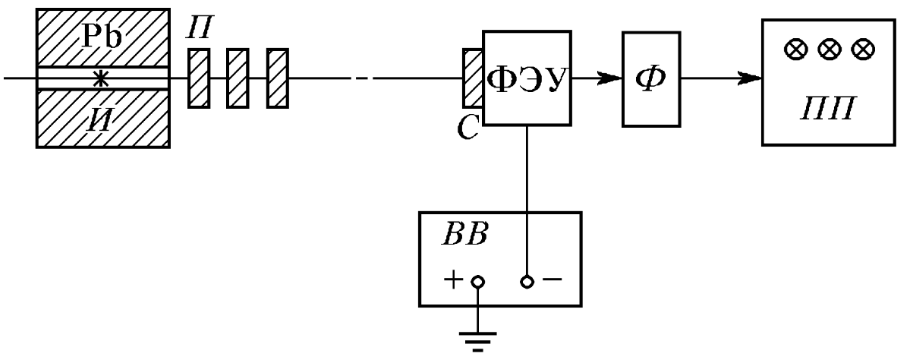
\includegraphics[scale=0.5]{img/1.png}
			\centering
			\caption{Схема установки.}
		\end{figure}
		На Рис. 1 изображена схема установки.
		Свинцовый коллиматор выделяет узкий почти параллельный пучок $\gamma$-квантов, проходящий через набор поглотителей П и регистрируемый сцинтилляционным счётчиком. 
		Сигналы от счётчика усиливаются и регистрируются пересчётным прибором ПП. 
		Высоковольтный выпрямитель ВВ обеспечивает питание сцинтилляционного счётчика. 
		Чтобы уменьшить влияние плохой геометрии, счётчик расположен на большим расстоянии от источника, поглотители имеют небольшие размеры, а так же устанавливаются на расстоянии друг от друга, чтобы испытавшие комптоновское рассеяние кванты с меньшей вероятностью могли в него вернуться.
	
	\section{Ход работы}
		
		\subsection{Оценка погрешностей}

			В начале эксперимента было измерено уоличество $\gamma$-квантов со свинцовой заглушкой и без.
			Результаты в расчете на одну секунду:
			\begin{equation}
				N_{\text{без}} = 11990 \hspace{10mm}
				N_{c} = 12 
			\end{equation}\par 
			По этим данным видно, что детектор воспринимает $\gamma$-излучение и оно меньше, чем внешний фон.\par
			Далее был проведен эксперимент по влиянию вторичных $\gamma$-лучей на результаты.
			Было изммерено количество частиц, регистрируемое при прохождении через 2 пластины алюминия в случае, когда они стояли на расстоянии в несколько сантиметров и в случае максимального расстояния.
			Результаты в расчете на одну секунду:
			\begin{equation}
				N_{standart} = 3763 \hspace{10mm}
				N_{max} = 3907 
			\end{equation}\par
			Также было измерено количство частиц после прохождения через пастину алюминия в случае, когда она стояла вплотную к детектору и в случае, когда вплотную к источнику.
			Таким образом мы сможем найти какой вклад дают вторичные $\gamma$-кванты.
			Полученное значение надо вычесть из эксперимента с двумя пластинами.
			Таким образом будет получена оценка погрешности, котрую вносят вторичные $\gamma$-кванты в остальных экспериментах.
			Поскольку далее образцы были расположены как можно бюлиже к источнику втоичные $\gamma$-кванты играют роль только при повторном рассеянии.
			\begin{equation}
				N_{\text{к источнику}} = 6285 \hspace{10mm}
				N_{\text{к детектору}} = 6527
			\end{equation}\par	
			Процент вторичных квантов в случае эксперимента с одной пластной:
			\begin{equation}
				err_{\text{прямые}} = \frac{\Delta N}{N} = 0.037
			\end{equation}\par
			Процент вторичных квантов в случае эксперимента с двумя пластинами:
			\begin{equation}
				err_{\text{рассеянные}} = \frac{\Delta N}{N} = 0.038
			\end{equation}\par
			Ошибка связанная с рассеянием вторичных $\gamma$-квантов:
			\begin{equation}
				err = err_{\text{рассеянные}} - err_{\text{прямые}} = 0.001
			\end{equation}\par
			Таким образом ошибка, связанная с взаимным расположением образцов, мала по сравнению с ошибкой, которая связана с расположением образцов относитеольно детектора.
			Поскольку образцы располагались близко к источнику, можно пренебречь ошибками, связанными с вторичными $\gamma$-квантами.
			В эксперимента присутствовала только случацная погрешность, которая не превышала 1 процент.\par
		
		\subsection{Расчет энергии}

			В эксперименте использовались пластины из различных материалов. 
			Размеры материалов:
			\begin{table}[h!]
				\centering
				\begin{tabular}{|l|l|}
				\hline
				Материал & Толщина {[}мм{]} \\ \hline
				Fe       & 10               \\ \hline
				Al       & 20               \\ \hline
				Pb       & 4.3              \\ \hline
				\end{tabular}
			\end{table}\par
	\newpage
			Результаты измерений поглощения $\gamma$-квантов:
			\begin{table}[h!]
				\centering
				\begin{tabular}{|l|l|l|}
				\hline
				Материал & Кол-во частиц & Время {[}c{]} \\ \hline
				Alx1     & 100000        & 15.91         \\ \hline
				Alx2     & 100000        & 26.57         \\ \hline
				Alx3     & 100000        & 40.09         \\ \hline
				Alx4     & 100000        & 61.58         \\ \hline
				Alx5     & 100000        & 98.39         \\ \hline
				Fex1     & 100000        & 17.58         \\ \hline
				Fex2     & 100000        & 36.36         \\ \hline
				Fex3     & 155177        & 100           \\ \hline
				Fex4     & 171080        & 200           \\ \hline
				Fex5     & 98418         & 200           \\ \hline
				Pbx1     & 100000        & 15.56         \\ \hline
				Pbx2     & 100000        & 30.02         \\ \hline
				Pbx3     & 100000        & 44.03         \\ \hline
				Pbx4     & 92550         & 100           \\ \hline
				Pbx5     & 115092        & 200           \\ \hline
				\end{tabular}
			\end{table}\par
			По полученным данным был построен график:
			\begin{figure}[h!]
                \centering
                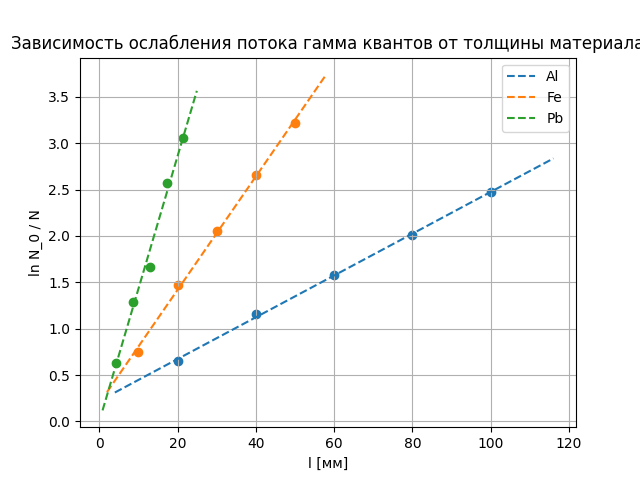
\includegraphics[width=15cm]{img/Graph.png}
                \caption{Схема экспериментальной установки}
                \label{graph1}
            \end{figure}
	\newpage
			По графику были расчитаны линейные коэффициенты ослабления:
			\begin{table}[h!]
				\centering
				\begin{tabular}{|l|l|l|}
				\hline
				Материал & Коэф наклона 1 / см & Погрешность \% \\ \hline
				Al       & 0.225               & 0.002          \\ \hline
				Fe       & 0.612               & 0.003          \\ \hline
				Pb       & 1.431               & 0.023          \\ \hline
				\end{tabular}
			\end{table}\par
			По таблице 4 были восстановлены примерные энергия $\gamma$-квантов:
			\begin{equation}
				E \approx 0.5 - 0.6 [\text{МэВ}]
			\end{equation} 
	
	\section{Вывод}
		
		В данной работе были измерены линейные коэффициенты поглащения для различных материалов.
		По ним была получена энергия $\gamma$-квантов одинаковая для всех экспериментов.
		 

\end{document}